\chapter{Introducci\'on a la L-simulaci\'on}
\label{sec:intro_logica}

mover a intro... y linkear con est capitulo...

No existe un acuerdo general sobre la representaci\'on b\'asica de
tanto la entrada y la salida del problema de GER; esto se maneja m\'as bien de manera ad-hoc
por cada nueva propuesta.

\cite{Krahmer2003} usan grafos dirigidos etiquetados en el contexto de este problema: los grafos son lo suficientemente abstractos 
para expresar un gran n\'umero de dominios y hay muchos algoritmos conocidos para tratar
con este tipo de estructuras. 

De hecho, no se trata de otra cosa que una representaci\'on alternativa de los modelos relacionales, usada t\'ipicamente }}
para proporcionar sem\'antica a los lenguajes formales como el de primer orden y l\'ogicas de orden superior, l\'ogicas modales, etc.


Exactamente debido a su generalidad, los grafos no definen por s\'i mismos, una \'unica noci\'on de igualdad. Cu\'ando decimos 
que dos nodos en el grafo pueden o no pueden ser
referenciados de forma \'unica en t\'erminos de sus propiedades? Esta pregunta s\'olo tiene sentido una vez que ya hemos 
fijado un cierto nivel de expresividad el cual determina cuando dos grafos, o dos elementos en el mismo gr\'afo, son equivalentes.

La expresividad se puede formalizar usando las relaciones estructurales de los grafos (isomorfismos, etc.) o, alternativamente, 
lenguajes l\'ogicos. 

%Ambas formas se presentan en Secci\'on \ref{sec:estructurales}, donde tambi\'en 
Discutiremos la noci\'on de impacto de expresividad 
en los casos que el problema GRE tiene soluci\'on; la complejidad computacional de los algoritmos GER involucrados; 
y la complejidad computacional del problema de la realizaci\'on. Luego investigamos el problema GER en t\'erminos de diferentes 
nociones de expresividad. 


\section{Seleccionando el lenguaje}

\newcommand{\nDog}{\mathit{dog}\xspace}
\newcommand{\nCat}{\mathit{cat}\xspace}
\newcommand{\aSmall}{\mathit{small}\xspace}
\newcommand{\aSniffing}{\mathit{sniffs}\xspace}
\newcommand{\nBreed}{\mathit{beagle}\xspace}

%\newcommand{\aLarge}{\mathit{large}\xspace}
%\newcommand{\nLeftOf}{\mathit{leftof}\xspace}
%\newcommand{\aRed}{\mathit{red}\xspace}
%\newcommand{\aYellow}{\mathit{yellow}\xspace}

Las estructuras relacionales son muy adecuadas para la representaci\'on de situaciones o escenas. La estructura relacional (tambi\'en llamado ``el modelo relacional'') es un conjunto no vac\'io de objetos -el dominio- junto con una colecci\'on de las relaciones, cada uno con una aridad fija.
Formalmente, asumimos un vocabulario fijo y finito (pero arbitrario) de
s\'imbolos de relaci\'on n-aria (las constantes y s\'imbolos de funci\'ones pueden ser representados como relaciones de aridad adecuada). 


Un modelo relacional $\+M$ es una tupla 
$\tup{\Delta,\interp{\cdot}}$ donde $\Delta$ es un conjunto no vac\'io, y
$\interp{\cdot}$ es una funci\'on de interpretaci\'on, esto es,
$\interp{r} \subseteq \Delta^n$ para todo s\'imbolo de relaci\'on $n$-aria tal que
$r$ est\'a en el vocabulario. $\+M$ es \emph{finito} cuando
$\Delta$ es finito.  El \emph{tama\~no} de un modelo $\+M$ es la suma
$\#\Delta + \#\interp{\cdot}$, donde $\#\Delta$ es la cardinalidad
de $\Delta$ y $\#\interp{\cdot}$ es la suma de todas las aridades de las
relaciones en $\interp{\cdot}$.

Vamos a presentar 2 ejemplos, uno en el que los tenemos agentes (perros y gatos),y otro en el que el dominio son cosas es decir, es de alguna manera est\'atico.

El primer ejemplo se muestra en la Figura~\ref{fig:cat-dog-1} en la cual hemos representado una escena
como un modelo relacional. Intuitivamente, $a$, $b$ y $d$ son dogs, mientras que 
$c$ y $e$ are cats;  $d$ es un small beagle;
 $b$ y $c$ son tambi\'en small.
 Leeremos $\aSniffing(d,e)$ como ``{\em $d$ is sniffing $e$}''.

 \begin{figure}
 \begin{center}
 \begin{tabular}{rcl}
$\Delta$               & = & $\cset{a,b,c,d,e}$\\
$\interp{\nDog}$      & = & $\cset{a,b,d}$\\
$\interp{\nCat}$      & = & $\cset{c,e}$\\
$\interp{\nBreed}$    & = & $\cset{d}$\\
$\interp{\aSmall}$    & = & $\cset{b,c,d}$\\
$\interp{\aSniffing}$ & = & $\cset{(a,a),(b,a),(c,b),(d,e),(e,d)}$
 \end{tabular}
\begin{picture}(120,50)
\put(0,-50){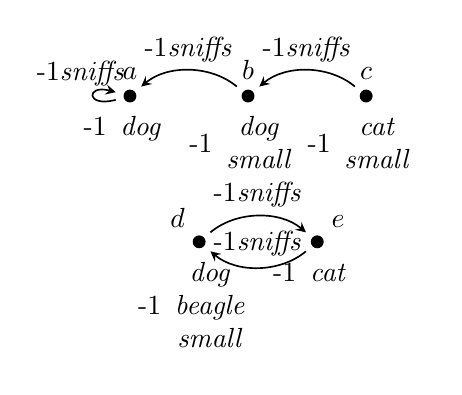
\begin{tikzpicture}
  [
    n/.style={circle,fill,draw,inner sep=1.5pt,node distance=1.5cm},
    aSniffing/.style={->, >=stealth, semithick, shorten <= 3pt, shorten >= 3pt},
  ]
 \node[n,label=above:$a$,label=below:{\relsize{-1}$\begin{array}{c}\nDog\end{array}$}] (a) {};

 \node[n,label=above:$b$,label=below:{\relsize{-1}$\begin{array}{c}\nDog\\ \aSmall \end{array}$}, right of=a] (b) {};

 \node[n,label=above:$c$,label=below:{\relsize{-1}$\begin{array}{c}\nCat\\ \aSmall\end{array}$}, right of=b] (c) {};

 \node[n,label=above left:$d$,label=below:{\relsize{-1}$\begin{array}{c}\nDog\\ \nBreed\\  \aSmall \end{array}$}, below of=a,xshift=25pt,yshift=-10pt] (d) {};

 \node[n,label=above right:$e$,,label=below:{\relsize{-1}$\begin{array}{c}\nCat\end{array}$},right of=d] (e) {};

 \draw [aSniffing,loop left] (a) to node[above,xshift=-5pt]{\relsize{-1}$\aSniffing$} (a);

 \draw [aSniffing,bend right=40] (b) to node[auto,swap]{\relsize{-1}$\aSniffing$} (a);

 \draw [aSniffing,bend right=40] (c) to node[auto,swap]{\relsize{-1}$\aSniffing$} (b);

 \draw[aSniffing, bend left=40] (d) to node[auto]{\relsize{-1}$\aSniffing$} (e);
 \draw[aSniffing, bend left=40] (e) to node[auto,swap]{\relsize{-1}$\aSniffing$} (d);

 \end{tikzpicture}}
 \end{picture}

 \end{center}
 \caption{Representaci\'on de escenas de Graph $\+S$.\label{fig:cat-dog-1}}
 \end{figure}





El segundo ejemplo se muestra en la Figura~\ref{grafo-GRE3D7-stimulus_b} en el que hemos representado el Contexto \ref{GRE3D7-stimulus1} 
como un modelo relacional. $e_1$,$e_3$,$e_5$, son 'ball', $e_2$, $e_6$ y $e_7$, son 'cube', mientras que 
$e_1$, $e_3$ y $e_6$ son 'yellow', $e_2$, $e_4$, $e_5$, $e_7$ son 'red';
%Para las relaciones tenemos $\Ontop(e_3,e_2)$ como ``{\em $e_3$ on top of $e_2$}''.
%$\Rightof(e_4,e_5)$, $\Rightof(e_6,e_7)$, $\Lefttof(e_5,e_4)$,$\Leftof(e_7,e_6)$. $e_4$ y $e_5$ son 'large', los dem\'as 'small'.

\begin{figure}
\begin{flushleft}
\begin{tabular}{rcl}
$\Delta$              & = & $\cset{e_1,e_2,e_3,e_4,e_5,e_6,e_7}$\\
$\interp{\aRed}$      & = & $\cset{e_2,e_4,e_5,e_7}$\\
$\interp{\aYellow}$   & = & $\cset{e_1,e_3,e_6}$\\
$\interp{\nBall}$     & = & $\cset{e_1,e_3,e_6}$\\
$\interp{\nCube}$     & = & $\cset{e_2,e_4,e_7}$\\

$\interp{\aSmall}$    & = & $\cset{e_1,e_2,e_3,e_6,e_7}$\\
$\interp{\aLarge}$    & = & $\cset{e_4,e_5}$\\

$\interp{\nRightof}$   & = & $\cset{(e_4,e_5),(e_6,e_7)}$\\
$\interp{\nLeftof}$    & = & $\cset{(e_5,e_4),(e_7,e_6)}$\\
$\interp{\nOntop}$     & = & $\cset{(e_3,e_2)}$\\

 \end{tabular}
\begin{picture}(120,50)
\put(0,-50){\begin{tikzpicture}
  [
    n/.style={circle,fill,draw,inner sep=1.5pt,node distance=1.5cm},
		 aArrow/.style={->, >=stealth, semithick, shorten <= 1pt, shorten >= 1pt},
    %aSniffing/.style={->, >=stealth, semithick, shorten <= 3pt, shorten >= 3pt},
  ]
%\begin{tikzpicture}
%  [
%    n/.style={circle,fill,draw,inner sep=3pt,node distance=2cm},
%    aArrow/.style={->, >=stealth, semithick, shorten <= 1pt, shorten >= 1pt},
%  ]
 \node[n,label=above:$e_1$,label=below:{
    \relsize{-2}$\begin{array}{c}
      \nSmall\\[-3pt] 
      \nYellow \\[-3pt] 
      \nBall\end{array}$}] (a) {};
 \node[n,label=above:$e_2$,label=below:{
    \relsize{-2}$\begin{array}{c}     
      \nSmall\\[-3pt] 
      \nRed\\[-3pt] 
      \nCube\end{array}$}, right of=a] (b) {};
 \node[n,label=below:$e_3$,label=above:{
    \relsize{-2}$\begin{array}{c}
      \nTop\\[-3pt]      
      \nSmall\\[-3pt] 
      \nYellow\\[-3pt] 
      \nBall\end{array}$}, above of=b] (c) {};
 \node[n,label=right:$e_4$,label=left:{
    \relsize{-2}$\begin{array}{c}
      \nLarge\\[-3pt] 
      \nRed\\[-3pt] 
      \nCube\end{array}$}, right of=b] (d) {};
 \node[n,label=left:$e_5$,label=below:{
    \relsize{-2}$\begin{array}{c}
      \nLarge\\[-3pt] 
      \nRed\\[-3pt] 
      \nBall\end{array}$}, right of=d] (e) {};
 \node[n,label=right:$e_6$,label=left:{
    \relsize{-2}$\begin{array}{c}
      \nSmall\\[-3pt] 
      \nYellow\\[-3pt] 
      \nCube\end{array}$}, right of=e] (f) {};
 \node[n,label=left:$e_7$,label=below:{
    \relsize{-2}$\begin{array}{c}
      \nSmall\\[-3pt]
      \nRed\\[-3pt] 
      \nCube\end{array}$},  right of=f] (g) {};
 \draw [aArrow,bend right=40] (b) to node[auto,swap]{\relsize{-3}$\nBelow$} (c);
 \draw [aArrow,bend right=40] (c) to node[auto,swap]{\relsize{-3}$\nOntop$} (b);
 \draw [aArrow,bend right=40] (d) to node[auto,swap]{\relsize{-3}$\nLeftof$} (e);
 \draw [aArrow,bend right=40] (e) to node[auto,swap]{\relsize{-3}$\nRightof$} (d);
 \draw [aArrow,bend right=40] (f) to node[auto,swap]{\relsize{-3}$\nLeftof$} (g);
 \draw [aArrow,bend right=40] (g) to node[auto,swap]{\relsize{-3}$\nRightof$} (f);
 \draw[dotted] (-0.5,-1.1) rectangle (8,2.6);

% \end{tikzpicture}
%\caption{Grafo del contexto \ref{GRE3D7-stimulus}}
%\label{grafo-GRE3D7-stimulus_b}
%\end{figure}
 \end{tikzpicture}}
 \end{picture}
 \end{flushleft}
 \caption{Representaci\'on del Contexto \ref{GRE3D7-stimulus1}}
 \label{grafo-GRE3D7-stimulus_b}
 \end{figure}


Los languajes l\'ogicos son \'utiles para la tarea de describir (formalmente) elementos de una estructura relacional. 

Por ejemplo, el lenguaje cl\'asico
de la l\'ogica de primer-orden (con desigualdad), \FOL, dado por:
$$
  \top \mid x_i \not\approx x_j \mid  r (\bar x) \mid \lnot \gamma \mid \gamma \land \gamma' \mid \exists x_i . \gamma
$$
%
donde $\gamma,\gamma' \in \FOL$,
$r$ es un s\'imbolo de relaci\'on $n$-aria y $\bar x$ es una tupla de $n$ variables.
Como es usual, $\gamma \lor \gamma'$ y $\forall x . \gamma$ son las versiones cortas de
$\lnot(\lnot\gamma \land \lnot\gamma')$ y $\lnot\exists x . \lnot\gamma$, respectivamente.
F\'ormulas de la forma $\top$, $x_i \not\approx x_j$ y $r(\bar
x)$ son llamados \emph{atomos}.%
  \footnote{%
    Por razones t\'ecnicas, incluimos el s\'imbolo de desigualdad symbol $\not \approx$ como
    primitivo. La igualdad puede ser definida usando negaci\'on.
  }
Dado un modelo relacional $\+M = \tup{\Delta,\interp{\cdot}}$ y una
f\'ormula $\gamma$ con variables libres%
\footnote{%
    W.l.o.g.\ asumimos que cada variable no puede aparecer libre y ligada a la vez, que una variable no esta ligada 2 veces,
    y que el \'indice de las variables crece en la f\'ormula de izquierda a derecha.%
}
entre $x_1\ldots x_n$, inductivamente definimos la \emph{extensi\'on} o
\emph{interpretaci\'on} de $\gamma$ como el conjunto de $n$-tuplas
 $\interp{\gamma}^n \subseteq \Delta^n$ que satisface:

\begin{center}
\begin{tabular}{rcl@{\hspace{1cm}}rcl}
$\interp{\top}^n$ &$=$& $\Delta^n$
&
$\interp{x_i \not\approx x_j}^n$ &$=$& $\cset{\bar{a} \mid \bar{a} \,{\in}\, \Delta^n, a_i \neq a_j}$
\\
$\interp{\lnot\delta}^n$ &$=$& $\Delta^n \setminus \interp{\delta}^n$
&
$\interp{r (x_{i_1} \ldots x_{i_k})}^n$ & $=$&$\cset{\bar{a} \mid \bar{a} \,{\in}\, \Delta^n, (a_{i_1} \ldots a_{i_k}) {\in} \interp{r}}$
\\
$\interp{\delta \land \theta}^n$ &$=$& $\interp{\delta}^n \cap \interp{\theta}^n$
&
$\interp{\exists x_{l}.\delta}^n$ &$=$& $\cset{\bar a \mid \bar a  e  \in \interp{\delta'}^{n+1}\ \text{for some $e$}}$
\end{tabular}
\end{center}
%
donde $1 \le i,j, i_1, \ldots, i_k \le n$, $\bar{a} = (a_1\ldots
a_n)$, $\bar{a}e = (a_1\ldots a_n,e)$ y $\delta'$ son
obtenidos reeplazando todas las ocurrencias de $x_l$ en $\delta$ por
$x_{n+1}$. 
%Cuando la cardinalidad de las tuplas involucradas en el contexto es conocida 
%escribiremos $\interp{\gamma}$ en lugar de
%$\interp{\gamma}^n$.

Con una sintaxis y sem\'antica de un lenguaje en mente, podemos formalmente definir el problema de L-GRE para un conjunto target de elementos T %(ligeramente adaptaremos la definici\'on en ~\cite{arec2:2008:Areces}):

\medskip
\noindent
{\small
\begin{center}
\begin{tabular}{ll} \hline
\multicolumn{2}{l}{
\textsc{Problema $\gL$-GRE }}\\ \hline
\ \ Input: & un model $\gM=\tup{\Delta,\interp{\cdot}}$ y un conjunto target no vac\'io $T \subseteq \Delta$.\\
\ \ Output: & una f\'ormula $\varphi \in \gL$ tal que
$\interp{\varphi} = T$ si existe, y $\bot$ caso contrario.\\ \hline
\end{tabular}
\end{center}}
Cuando el output es no $\bot$, decimos que $\phi$ es una
\emph{expresi\'on referencial en $\+L$ (ER-$\+L$) para $T$ en $\+M$}.

La salida de el problema $\+L$-GRE es una f\'ormula de
$\+L$ cuya interpretaci\'on en el modelo de input $\gM$ es el conjunto target, si
esa f\'ormula existe. 


% Esta definici\'on aplica incluso a la GRE para
%objetos  de el dominio teniendo un conjunto singleton como target.

Consideramos solo modelos relacionales con s\'imbolos de relaciones unarios y binarios, usaremos $p$ para las proposiciones (propiedades) y $r$ para los s\'imbolos de relaci\'on binarias.


Seleccionando el lenguaje apropiado...

Dado un modelo M, podr\'ia haber un infinito n\'umero de f\'ormulas que de forma \'unica
describan al target (incluso f\'ormulas que no son l\'ogicamente equivalentes podr\'ian tener
la misma interpretaci\'on una vez al modelo este fijo). 


Por ejemplo en el Contexto \ref{GRE3D7-stimulus1} \Large \Ball y \Red \Ball son diferentes f\'ormulas pero tienen la misma interpretaci\'on en $+M$.

Como es bien conocido en la comunidad de generaci\'on autom\'atica de lenguaje natural, diferentes
realizaciones del mismo contenido podr\'ian dar lugar a expresiones referenciales que son m\'as o menos
apropiadas en el contexto dado. 

Argumentamos que la generaci\'on de contenido usando lenguajes con diferente poder expresivo puede tener un impacto en la estapa posterior
de realizaci\'on sint\'actica (surface realization).

F\'ormulas que identifican a $b$ en nuestro primer ejemplo

\begin{table}
$$
\begin{array}{cl}
 \gamma_1: & \nDog(x) \land \aSmall(x) \land
   \exists y . (\aSniffing(x,y) \land \nDog(y))\\[3pt]
  %
  \gamma_2: & \nDog(x) \land \aSmall(x) \land
  \forall y . (\neg \nCat(y) \lor \neg \aSniffing(x,y))\\[3pt]
  %
  \gamma_3: & \nDog(x) \land
  \exists y . (x \not\approx y \land \nDog(y)  \land \aSniffing(x,y))\\[3pt]
  %
  \gamma_4: & \nDog(x) \land
  \exists y . (\nCat(y) \land \aSmall(y) \land \aSniffing(y,x))
  %
 \end{array}
$$
\caption{Descripciones alternativas para el objeto $b$ en el modelo mostrado en Figura~\ref{fig:cat-dog-1}.}\label{tab:gammas}
\end{table}

Restringiendo la determinaci\'on de contenido a FO-, aseguramos que f\'ormulas como  $\gamma_2$ no se generar\'an. Si prohibimos el distinto del lenguaje  $\gamma_3$ tambi\'en queda exclu\'ida.

El hecho de que el lenguaje de representaci\'on utilizado tiene un impacto sobre la determinaci\'on de contenido es obvio, pero no ha recibido la atenci\'on que merece. Areces et al. [1] usaron diferentes l\'ogicas de descripci\'on (una familia de lenguajes formales utilizado en representaci\'on del conocimiento, vea [2]) para clasificar y dar un marco formal para
trabajo previo sobre GRE. Vamos a presentar r\'apidamente algunas de estos lenguajes ya que los mencionaremos en las siguientes secciones. Usando l\'ogicas de descripci\'on en lugar de fragmentos de FO es s\'olo una cuesti\'on de notaci\'on, como la mayor\'ia de l\'ogicas descriptivas se pueden ver
fragmentos como impl\'icitas de FO. Por ejemplo, el lenguaje de la l\'ogica de descripci\'on ALC, se define sint\'acticamente como el conjunto de f\'ormulas,
$$
\top \mid p \mid \neg \gamma \mid \gamma \wedge \gamma' \mid  \exists r. \gamma
$$
(donde $p$ es un s\'imbolo proposicional, $r$ s\'imbolo relacional binario, y $\gamma,\gamma' \in \ALC$) corresponde al fragmento sint\'actico de
\FOL sin $\not\approx$, como es mostrado por la traducci\'on est\'andar $\st_x$:

\begin{center}
\begin{tabular}{rcl@{\hspace{1cm}}rcl}
$ \st_{x_i}(\top)$ &$=$& $\top$
&
$\st_{x_i}(\gamma_1 \land \gamma_2)$ &$=$& $\st_{x_i}(\gamma_1) \land \st_{x_i}(\gamma_2)$
\\
  $\st_{x_i}(p)$ &$=$& $p(x_i)$
&
$\st_{x_i}(\exists r . \gamma)$ &$=$& $\exists x_{i+1} . (r(x_i,x_{i+1}) \land \st_{x_{i+1}}(\gamma))$
\\
 $\st_{x_i}(\lnot \gamma)$ &$=$& $\lnot\st_{x_i}(\gamma)$
&
\end{tabular}
\end{center}

En efecto, dado un modelo relacional $\+M$, la extensi\'on de una f\'ormula \ALC en M coincide exactamente con la extensi\'on de $\st_{x_1}(\varphi)$ (v\'ease, por ejemplo, ~\cite{baad:desc03}). Gracias
a este resultado, para cualquier f\'ormula $\varphi$ de \ALC y sus sublenguajes podemos definir $\interp{\varphi} = \interp{\st_{x_1}(\varphi)}$.
 Volviendo a nuestro ejemplo anterior, mediante la restricci\'on de contenido
generaci\'on en f\'ormulas $\ALC$ (o equivalentemente, el fragmento correspondiente de \FOL)
evitar\'iamos f\'ormulas como
$\gamma_3$ (sin igualdad) y
$\gamma_4$ (aparece cuanti elemento ed
siempre en segunda posici\'on de argumento).
Generaci\'on se discute en ~\cite{AKS08}, en t\'erminos de diferentes l\'ogicas de descripci\'on como \ALC
y \EL (\ALC sin negaci\'on). Vamos a ampliar los resultados en ese papel, con-
Sidering por ejemplo \ELAN (\ALC con la negaci\'on permitida s\'olo frente a relaciones unarias), pero, en general, nosotros tomamos un enfoque modelo te\'orico y argumentamos que la cuesti\'on principal no es si se debe utilizar una u otra (descripci\'on l\'ogica para la generaci\'on de contenido, sino que son el diferencias sem\'antica a tener en cuenta. Esto no solo determina el formalismo l\'ogico requerido sino tambi\'en impacta tanto en la determinaci\'on de contenido como en los problemas de realizaci\'on sint\'actica. Cada
lenguaje l\'ogico puede ser visto como un compromiso entre la expresividad, realizabilidad y complejidad computacional. La selecci\'on apropiada para una tarea GRE particular, debe depender del contexto actual




Para el segundo ejemplo: \\
Supongamos que queremos identificar a $e_5$ del Contexto \ref{GRE3D7-stimulus-conLetras}, las siguientes son f\'ormulas que identifican a un\'ivocamente a $e_5$ en el contexto considerado.

\begin{table}
$$
\begin{array}{cl}
 \gamma_1: & \aRed(x) \land \nBall(x)\\[3pt]
  %
 \gamma_2: & \aLarge(x) \land \nBall(x)\\[3pt]
  %
 \gamma_3: & \nLarge(x) \land \aRed(x) \land \nBall(x)\\[3pt]
  %
 \gamma_4: & \nLarge(x) \land \aRed(x) \land \nBall(x) \land
   \exists y . (\nRightof(x,y) \land \aLarge(y) \land \aRed(y) \land \nCube(y))\\[3pt]
  %ex1
 \gamma_5: & \nLarge(x) \land \aRed(x) \land \nBall(x) \land
  \forall y . (\neg \nBall(y) \lor \neg \nRightof(x,y))\\[3pt]
  %ex 2
 \gamma_6: & \nLarge(x) \land \aRed(x) \land \nBall(x) \land
  \exists y . (x \not\approx y \land \nCube(y) \land \nRightof(x,y))\\[3pt]
  %ex 3
 \gamma_7: & \nLarge(x) \land \aRed(x) \land \nBall(x) \land
  \exists y . (\nCube(y) \land \aRed(y) \land \nLeftof(y,x))
  %ex 4
 \end{array}
$$
\caption{Descripciones alternativas para el objeto $e_5$ del Contexto~\ref{GRE3D7-stimulus-conLetras}.}\label{tab:gammas}
\end{table}

Notar que $\gamma_2$ y $\gamma_3$ son m\'inimas, es decir no se puede dar una f\'ormula m\'as corta que esas.
$\gamma_4$ se puede realizar como ``Large red ball right-of large red cube''. Esta f\'ormula junto con $\gamma_1$, $\gamma_2$ y $\gamma_3$ son caracterizadas como f\'ormulas positivas, conjuntivas y existenciales (no contienen negaci\'on y solo tienen conjunciones y cuantificadores existenciales), este tipo de f\'ormulas son las que m\'as se encuentran en corpus ~\cite{viethen06:_algor_for_gener_refer_expres,deemter06:_build_seman_trans_corpus_for,gre3d3}.

Bueno, pero entonces podemos elegir otra l\'ogca cuyo lenguaje este restringido a las ER que queremos generar.

Restringiendo la determinaci\'on de contenido a FO-, aseguramos que f\'ormulas como  $\gamma_5$ no se generar\'an. 
Si prohibimos el distinto del lenguaje  $\gamma_6$ tambi\'en queda exclu\'ida.

%El hecho de que el lenguaje de representaci\'on utilizado tiene un impacto sobre la determinaci\'on de contenido es obvio, 
%pero no ha recibido la atenci\'on que merece. 
%Areces et al. [1] usaron diferentes l\'ogicas de descripci\'on (una familia de lenguajes formales utilizado en 
%representaci\'on del conocimiento, vea [2]) para clasificar y dar un marco formal para
%trabajo previo sobre GRE. 

Usar l\'ogicas de descripci\'on en lugar de fragmentos de FO es s\'olo una cuesti\'on de notaci\'on, como la mayor\'ia de l\'ogicas 
descriptivas se pueden ver como
fragmentos de FO. Por ejemplo, el lenguaje de la l\'ogica de descripci\'on ALC, se define sint\'acticamente como el conjunto de f\'ormulas,
$$
\top \mid p \mid \neg \gamma \mid \gamma \wedge \gamma' \mid  \exists r. \gamma
$$
(donde $p$ es un s\'imbolo proposicional, $r$ s\'imbolo relacional binario, y $\gamma,\gamma' \in \ALC$) corresponde al fragmento 
sint\'actico de
\FOL sin $\not\approx$, como es mostrado por la traducci\'on est\'andar $\st_x$:

\begin{center}
\begin{tabular}{rcl@{\hspace{1cm}}rcl}
$ \st_{x_i}(\top)$ &$=$& $\top$
&
$\st_{x_i}(\gamma_1 \land \gamma_2)$ &$=$& $\st_{x_i}(\gamma_1) \land \st_{x_i}(\gamma_2)$
\\
  $\st_{x_i}(p)$ &$=$& $p(x_i)$
&
$\st_{x_i}(\exists r . \gamma)$ &$=$& $\exists x_{i+1} . (r(x_i,x_{i+1}) \land \st_{x_{i+1}}(\gamma))$
\\
 $\st_{x_i}(\lnot \gamma)$ &$=$& $\lnot\st_{x_i}(\gamma)$
&
\end{tabular}
\end{center}

En efecto, dado un modelo relacional $\+M$, la extensi\'on de una f\'ormula \ALC en $\+M$ coincide exactamente con la extensi\'on
 de $\st_{x_1}(\varphi)$ (v\'ease, por ejemplo, ~\cite{baad:desc03}). Gracias
a este resultado, para cualquier f\'ormula $\varphi$ de \ALC y sus sublenguajes podemos definir 
$\interp{\varphi} = \interp{\st_{x_1}(\varphi)}$.




 Volviendo a nuestro ejemplo anterior, mediante la restricci\'on de la generaci\'on de contenido
a f\'ormulas de $\ALC$ (o equivalentemente, el fragmento correspondiente de \FOL)
evitar\'iamos f\'ormulas como
$\gamma_5$ (sin igualdad) y

$\gamma_4$ (aparece cuanti elemento ed
siempre en segunda posici\'on de argumento). ESTE EJ NO LO PUSE... ver si consigo alguno interesante


%Generaci\'on se discute en ~\cite{AKS08}, en t\'erminos de diferentes l\'ogicas de descripci\'on como \ALC
%y \EL (\ALC sin negaci\'on). Vamos a ampliar los resultados en ese papel, consideando por ejemplo \ELAN 
%(\ALC con la negaci\'on permitida s\'olo frente a relaciones unarias), pero, en general, nosotros tomamos un enfoque modelo te\'orico y argumentamos que la cuesti\'on principal no es si se debe utilizar una u otra (descripci\'on l\'ogica para la generaci\'on de contenido, sino que son el diferencias sem\'antica a tener en cuenta. Esto no solo determina el formalismo l\'ogico requerido sino tambi\'en impacta tanto en la determinaci\'on de contenido como en los problemas de realizaci\'on sint\'actica. Cada
%lenguaje l\'ogico puede ser visto como un compromiso entre la expresividad, realizabilidad y complejidad computacional. La selecci\'on apropiada para una tarea GRE particular, debe depender del contexto actual





----
Argumento a favor EL
----


  


%\section{}




